
\documentclass[openany]{XDBT}

\begin{document}

%%----------SURFACE----------%%

	%% Here you can fill your information:
	
	\title{西电本科毕业设计论文模板}
	%\rtitle{} %If your title is overflowed in a line, split it here. Or, ignore it. 
	\institute{计算机学院}
	\major{计算机科学与技术}
	\author{刘曜}
	\advisor{Google}
	%\class{}
	%\studentNumber{}
	\maketitle


%%----------PROLOGUE---------%%
	\frontmatter
	
\begin{abstract}

这篇文章是这个\LaTeX{}~模板的测试,我顺便写一点关于这个模板的用法。就像你现在看到的,这是一个摘要。

依据学校给的要求(已经放在附录A里了),章标题要求黑体,三号,居中;节标题要求四号,居中;其他各级标题都是小四号,黑体,居左;正文小四号,宋体,中文段落空两个字。

大概就是这些,关键字要求3-5个,中间用空格分开。

\keywords{西电~~论文~~毕业设计~~模板}
\end{abstract}

\begin{enabstract}

This is an abstract in English. I don't want to translate the content above, just a sample~~So, that's end. 

\enkeywords{Xidian~~University~~Thesis~~Template}

\end{enabstract}

	\tableofcontents

%%----------MAIN PART--------%%
	\mainmatter
	\pagestyle{content}
	\chapter{模板介绍}
\label{chap:introduction}

这个模板为2017年毕业而诞生~

因为我想用\LaTeX{}~写毕设,放寒假这几天趁小伙伴都还没回来,抽时间先写个论文模板,顺便练一下\LaTeX{}~很多用法。

这个模板我参照了一点睿思上数院一个师兄(薛继龙)的模板,但宏结构跟他写的区别不小……顺便修复了一点他的小问题,然后我的这个模板可能更custom~

\section{系统环境}
我写这个模板的系统是linux(ubuntu 16.04),文档字符集UTF-8(师兄那个是GB18030,在windows上可能不会乱码,在linux上得改配置不然会乱码)。

其次,\LaTeX{}~环境我记得我是很久以前直接装的texlive-full,然后装了个latex-cjk-chinese,好像再也没有装过其他的了,文档最终用的xelatex跑的,所以一般情况下只要装的一样,运行时不会出现少包少字体的情况。

\section{拿到模板改哪些}
首先目录结构和你需要关注的文件有这些:
\begin{itemize}
\item main.tex: 模板主文件,统筹模板的环境,和添加相应的章节,最后也是运行它。
\item partial: 这个文件夹里面*.tex的文件都是需要你自己写的(每一章写在不同文件里,可自己添加),只需要会一点点latex语法就能搞定,不需要关注版式和字体之类的,只关注内容写什么。自己添加的*.tex需要你在main.tex文件里适当的位置用$\backslash$include命令包含进去,写对路径就行。
\item graphics: 这个文件全都是图形图像文件,必须是.eps后缀,其他格式图片你可以转成.eps再放进去。有个网站很好很强大能转换,但是好像需要翻墙:\href{http://www.tlhiv.org/rast2vec/}{http://www.tlhiv.org/rast2vec/}
\item XDBT.cfg: 这里面定义了一堆常量,你可以自定义更改,但我已经按照学校要求写好了,应该不用再打开更改了。
\item XDBT.cls: 这就是宏文件,其实不用打开看,已经基本弄好了。如果想微调模板板式、字体、颜色之类的,可以在这里调,我写了比较粗糙的注释。
\item 其他文件你大部分时候都不需要关注是啥。
\end{itemize}

其次,你可能注意到了,学校也要求到,页要分左手和右手方向,奇数页左边留白多,偶数页右边留白多。有的页需要从奇数页开始(比如最后的致谢),如果它刚好是在偶数页,你可以在它之前的那一个部分的结尾加一个$\backslash$cleardoublepage用来加一个空白页。

\section{版式对齐}

现在的版式不会出现某一行太长了发生溢出的情况,因为我在XDBT.cls文件里加了几句话,主要是$\backslash$tolerance这个变量。

但现在会有一种状况,若有个特长的东西如http://www.penpineappleapplepen.com,就会让上一行的字间距特别大,就像这里的情况一样。这是无法避免的(起码我不知道)。此时就要求你能合理断句,或者在合适的地方写下比较长的部分。

师兄那个模板会出现行溢出的现象,就是写出去,像这个右侧一样
\begin{figure}[h]
 \centering
	\fbox{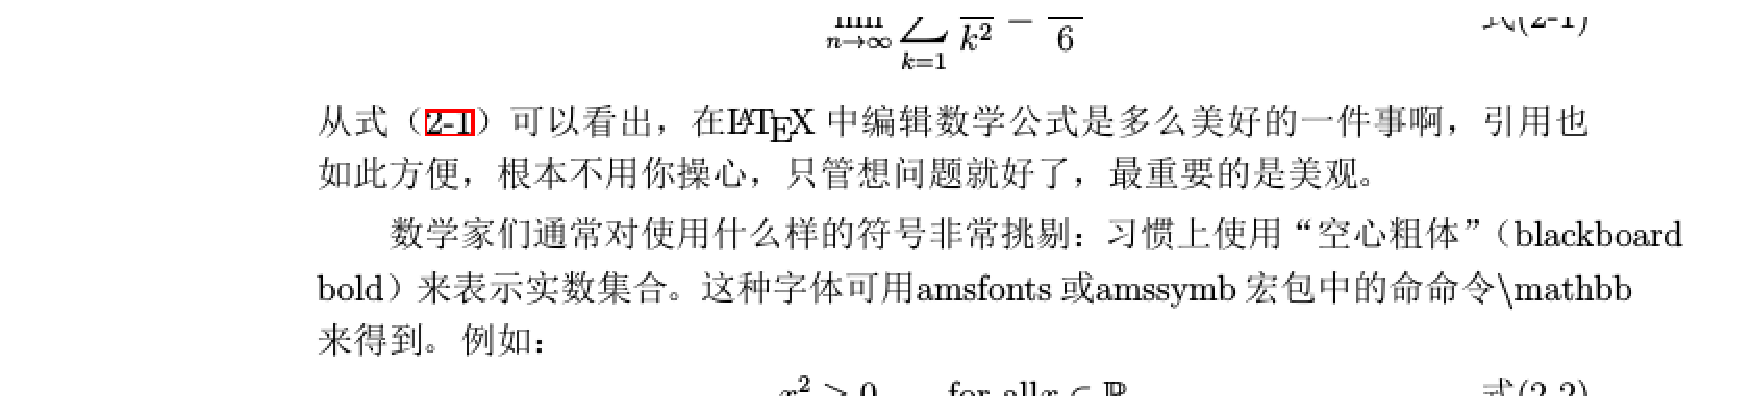
\includegraphics[width=1\textwidth]{overflow}}
 \caption{行溢出}
 \label{fig:amss1}
\end{figure}

这样的话,也是需要你在适当的地方换行。如果你想用他这种,自己写的时候稍微注意一下也可以,你只需要把上面那个变量注释掉就行了。

\section{版权问题}

尊重版权,保证自由,鼓励开源,不建议收费- -

GNU License

\section{问题反馈}

如果模板有问题,你可以自己改改,我也欢迎和我讨论交流:

\href{derektanko@gmail.com}{derektanko@gmail.com}

祝各位顺利毕业,升职加官,当CEO,娶白富美(or嫁高富帅),早得贵子,延续人类,(入土为安)。
	
\chapter{数学相关}
\label{chap:math}
我稍微写写关于数学相关的语法,测试一下模板是否运行正确。
\cite{mycite}。

\section{公式}

\begin{itemize}
    \item 行内的公式一般用\$和\$,这两个之间夹着你要写的内容,示例:这样的写法(顺便也把代码块的写法测试了- -,代码块的样式在XDBT.cls里面有定义)%
    \begin{lstlisting}
    $a^2+b^2=c^2$
    \end{lstlisting}
    会得到$a^2+b^2=c^2$
    \item 行间公式用\$\$和\$\$,示例:
    \begin{lstlisting}
    $$a^2+b^2=c^2$$
    \end{lstlisting}
    会得到$$a^2+b^2=c^2$$
    \item 还有带编号的公式,我就不写代码了,你可以去看这个模板源码,效果:
    \begin{equation}\label{eq:lim}
        a^2+b^2=c^2
    \end{equation}
\end{itemize}

\section{定理和定义}
同样不贴代码了,只有演示效果
\begin{thm}
我是一个小定理~
\end{thm}

\begin{thm}
我是另一个小定理,带公式的小定理~
\begin{equation}
    a^2+b^2=c^2
\end{equation}
\end{thm}

\begin{algo}
我是一个小算法~
\end{algo}






	
\chapter{表格图形}
\label{chap:tabfig}

\section{表格}
示例1,中间有竖线的:
\begin{center}
\begin{tabular}[t]{l|c}
    \hline
    姓名 & 战斗力 \\
    \hline
    习XX & 999 \\
    蛤XX & 9999 \\
    川普 & 0.1 \\
    \hline
\end{tabular}
\end{center}


示例2,中间没竖线的:
\begin{table}[htbp]
 \caption{\label{tab:test}示例表格}
 \centering
 \begin{tabular}{lcl}
  \toprule
    姓名 & 战斗力 \\
  \midrule
    习XX & 999 \\
    蛤XX & 9999 \\
    川普 & 0.1 \\
  \bottomrule
 \end{tabular}
\end{table}

\section{图形}
这玩意儿好像只能加eps的图,前面提到了,也给转换工具的网址了

示例:
\begin{figure}[h]
 \centering
 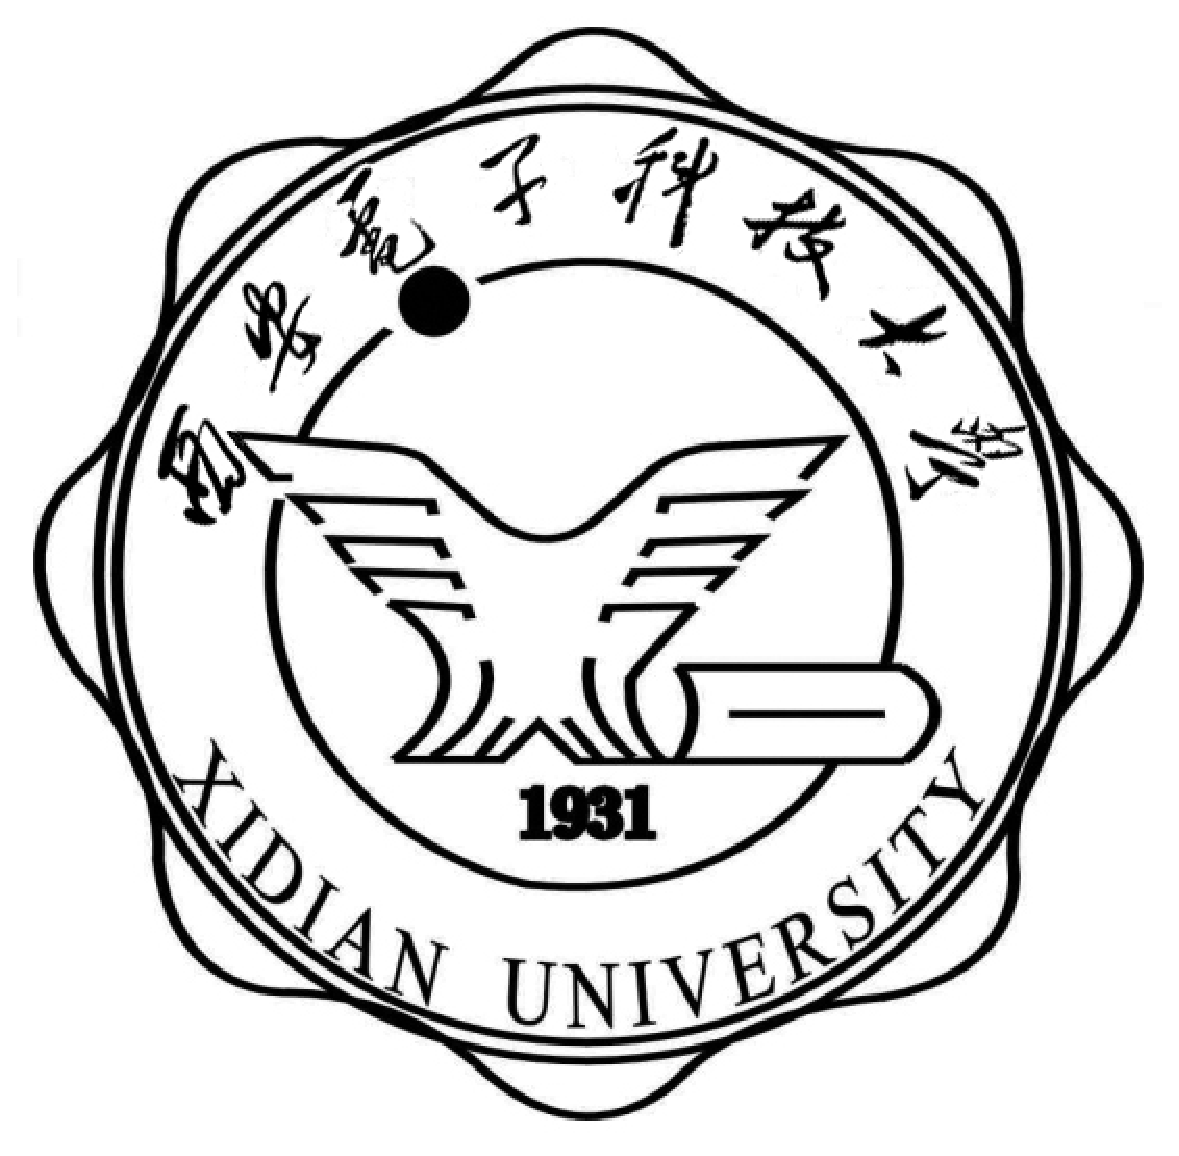
\includegraphics[width=0.3\textwidth]{xdSign}
 \caption{这是一个图片}
 \label{fig:amss1}
\end{figure}




	\appendix
\titleformat{\chapter}[hang]{\heiti\bfseries\center\zihao{3}}{附录{\thechapter}}{1em}{\zihao{3}}
	
\chapter[本科生毕业设计论文撰写规范]{西安电子科技大学本科生毕业设计论文撰写规范}
\label{chap:requires}
\section{毕业设计(论文)的总体要求}
撰写论文应简明扼要,一般不少于15000字(外语专业可适当减少,但不得少于10000单词,且须全部用外语书写)。

\section{毕业设计(论文)的编写格式}
每一章、节的格式和版面要求整齐划一、层次清楚。其中:
\begin{itemize}
  \item 论文用纸:统一用A4纸,与论文封皮,任务书,工作计划,成绩考核表一致。
  \item 章的标题:如:"摘要"、"目录"、"第一章"、"附录"等,黑体,三号,居中排列。
  \item 节的标题:如:"2.1  认证方案"、"9.5  小结"等,宋体,四号,居中排列。
  \item 正文:中文为宋体,英文为"Times News Roman",小四号。正文中的图名和表名,宋体,五号。
  \item 页眉:宋体五号,居中排列。左面页眉为论文题目,右面页眉为章次和章标题。页眉底划线的宽度为0.75磅。
  \item 页码:宋体小五号,排在页眉行的最外侧,不加任何修饰。
\end{itemize}

\section{毕业设计(论文)的前置部分}
毕业设计(论文)的前置部分包括封面、中英文摘要、目录等。
\subsection{封面及打印格式}
\begin{itemize}
  \item 学号:按照学校的统一编号,在右上角正确打印自己的学号,宋体,小四号,加粗。
  \item 题目:题目应和任务书的题目一致,黑体,三号。
  \item 学院、专业、班级、学生姓名和导师姓名职称等内容,宋体,小三号,居中排列。
\end{itemize}

\subsection{中英文摘要及关键词}
摘要是关于论文的内容不加注释和评论的简短陈述,具有独立性和自含性。它主要是
简要说明研究工作的目的、方法、结果和结论,重点说明本论文的成果和新见解。关键词
是为了文献标引工作从论文中选取出来用以表示全文主题内容信息的术语。
\begin{enumerate}
  \item 中文摘要,宋体小四号,一般为300字;英文摘要,"Times News Roman"字
体,小四号,一般为300个实词。摘要中不宜出现公式、非公用的符号、术语等。
  \item 每篇论文选取3 \~{} 5个关键词,中文为黑体小四号,英文为"Times News Roman"字体加粗,小四号。关键词排列在摘要的左下方一行,起始格式为:"\textbf{关键词}:
      "和"\textbf{Keyword:}"。具体的各个关键词以均匀间隔排列,之间不加任何分隔符号。
\end{enumerate}

\section{目录}
按照论文的章、节、附录等前后顺序,编写序号、名称和页码。目录页排在中英文摘要之后,主体部分必
须另页右面开始,全文以右页为单页页码。

\section{毕业设计(论文)的主体部分}
毕业设计(论文)的主体部分包括引言(绪论)、正文、结论、结束语、致谢、参考文献。
\subsection{绪论}
作为论文的开端,简要说明作者所做工作的目的、范围、国内外进展情况、前人研究成果、
本人的设想、研究方法等。
\subsection{正文} 为毕业设计(论文)的核心部分,包括理论分析、数据资料、实验方法、结果、本人的论点和结
论等内容,还要附有各种有关的图表、照片、公式等。要求理论正确、逻辑清楚、层次分明、文字流畅、数据真实可
靠,公式推导和计算结果无误,图表绘制要少而精。
\begin{description}
  \item[图] 包括曲线图、示意图、流程图、框图等。图序号一律用阿拉伯数字分章依序编码,如:图1.3、图2.11。每一图应有简短确切的
      图名,连同图序号置于图的正下方。图中坐标上标注的符号和缩略词必须与正文中一致。
  \item[表] 包括分类项目和数据,一般要求分类项目由左至右横排,数据从上到下竖列。分类项目横排中必须标明符号或单位,竖列的数据栏中不宜出现"同上" 、"同左"等类似词语,一律填写具体的数字或文字。表序号一律用阿拉伯数字分章依序编码,如:表2.5、表10.3。每一表应有简短确切的题名,
      连同表序号置于表的正上方。
  \item[公式] 正文中的公式、算式、方程式等必须编排序号,序号一律用阿拉伯数字分章依序编码,如:式(3-32)、式(6-21)。对于较长的公式,另行居中横排,只可在符号处(如:+、-、*、/、$<$、 $>$等)转行。公式序号标注于该式所在行(当有续行时,应标注于最后 一行)的最右边。连续性的公式在"="处排列整齐。大于999的整数或多于三位的小数,一律用半个阿拉伯数字符的小间隔分开;小于1的数应将0置于小数点之前。
  \item[计量单位] 单位名称和符号的书写方式一律采用国际通用符号。
\end{description}

\subsection{结论}
是对主体的最终结论,应准确、完整、精炼。阐述作者创造性工作在本研究领域的地位和作用,对存在的问题和不足应给予客观的说明,也可提出进一步的设想。

\subsection{致谢}
对协助完成论文研究工作的单位和个人表示感谢。

\subsection{参考文献}
在学位论文中引用参考文献时,引出处右上角用方括号标注阿拉伯数字编排的序号(必须与参考文献一致)。参考文献的排列格
式分为:
\begin{description}
  \item[专著类的文献] [序号]  作者 . 专著名称.  版本. 出版地:出版者,出版年. 参考的页码。
  \item[期刊类的文献] 作者 . 文献名. 期刊名称.  年 , 月,  卷(期). 页码。
\end{description}
其中作者采用姓在前、名在后的形式。当作者超过三个时,只著录前三个人,其后
加"等"字即可。

\section{毕业设计(论文)的附录部分}
附录是作为学位论文主体的补充,包括下列内容:
\begin{enumerate}
  \item 正文中过于冗长的公式推导;
  \item 为读者阅读方便所需要的辅助性的数学工作或带有重复性的图表;
  \item 由于过分冗长而不宜在正文中出现的计算机程序清单;
  \item 对于一般读者并非必要阅读,但对本专业同行有参考价值的资料。
  \item 附录编于正文后,与正文连续编页码,每一附录均另页起。
  \item 附录依次用大写正体A,B,C……编序号,黑体,三号。如:附录A。
  \item 附录中的图、表、式、参考文献等与正文分开,用阿拉伯数字另行编序号,注意在数码前冠以附录的
      序码。如:图A1;表B2;式(C-3);文献[D5]。
\end{enumerate}
\section{毕业设计(论文)的打印规格}
论文正文页面和版面的设置规格:论文正文双面打印,为了便于装订、复制,要求每页纸的四周留有足够的空白边缘。以WORD97为例:

页面设置数据为:上3厘米、下2厘米、内侧3厘米、外侧2厘米;装订线 -- 1厘米;页眉  - 2厘米;  页脚 - 1厘米。

版面设置数据为:文字的行间距 - 1. 5倍 ;  公式的行间距 - 1. 5倍字符间距 - 标准;页码数据-对称页边距。

\section{毕业设计(论文)的装订说明}
毕业设计(论文)要求以A4纸的标准,按照下列顺序装订。外文资料翻译原文及译文另册装订,格式参照论文对应内容格式要求。

\begin{enumerate}
  \item 封面
  \item 任务书
  \item 工作计划
  \item 中期检查表
  \item 成绩考核登记表
  \item 中、外论文摘要
  \item 目录
  \item 引言
  \item 论文
  \item 结论
  \item 结束语
  \item 参考文献
  \item 附录
\end{enumerate}












%%----------ACCESSORY--------%%
    \backmatter
    
\begin{thanks}

这就是一个致谢页面,通常你要在这里把你身边认识的人都问候一遍。举个例子:

谢谢祖国,谢谢陕西,谢谢长安,谢谢爸爸,谢谢妈妈,谢谢西电校园,谢谢西电所有老师,谢谢西电所有同学,谢谢楼管,谢谢综合楼,谢谢西电流浪狗,谢谢西电流浪猫,谢谢西电其他流浪的动物,谢谢lol,谢谢DotA,谢谢炉石,谢谢其他游戏,谢谢麒麟臂,谢谢大家,让我在西电这个校园活着度过了这四年,god bless you,今当远离,临表涕零,不知谓何,特此鸣谢。

哦,论文啊,已经写完了,我能毕业了吧?谢谢谢谢审核老师,祝你鸡年大吉!

......

\vskip 18pt

2017-01-17

\end{thanks}

\cleardoublepage

    
\fontsize{10.5pt}{10.5pt}\selectfont
\begin{thebibliography}{10}

\bibitem{mycite}
这是一个引用的示例
\newblock {附件里有个关于数学语法的详细讲解.pdf}.
\newblock (2017)


\end{thebibliography}


\end{document}